\documentclass[12pt,a4paper]{article}

\usepackage[left=20mm, right=20mm, top=20mm]{geometry} % to set up page formatting
\usepackage[skip=10pt]{parskip} % spacing in between paragraphs
\usepackage{graphicx} % Required for inserting images
\usepackage{amsmath} % Required for flexibility in mathematical equations
\usepackage{amssymb} % Required for certain math symbols e.g. E[.]
\usepackage{natbib} % Required for bibliography and citations
\usepackage{enumitem} % Required to remove gap between items in list
\usepackage{tikz} % Required to build tikz diagrams
\usepackage{xcolor} % to access colors in tikz diags
\usepackage{hyperref} % for web links

\title{Multi-fidelity modelling and optimisation with applications in long-term public sector capacity planning: ten month PhD review}
\author{Graham Burgess}
\date{November 2024}

\begin{document}
%
\maketitle
%
\section{Introduction}
%
Long-term capacity planning is a problem for organisations worldwide, especially for public sector bodies who must meet basic public needs with tight financial budgets. Examples of such problems arise in housing, healthcare and prisons. In housing, decision makers must split their resources between emergency shelter and permanent social housing to alleviate homelessness. In healthcare, planners must balance the need for critical and non-critical care services when designing new hospitals. In prisons, capacity must be sufficient to avoid needing to release prisoners early but not so high as to risk costly unused capacity. 

Operational research methods offer helpful tools to support such public sector decision-making. Optimisation helps by looking for a feasible solution which performs best across a set of alternative feasible solutions. To do this, a model of the system's performance is needed, and the quality of the model affects the quality of the subsequent optimisation results. The flow of people through public services can often be modelled as a queue. For example, in a homeless care system, individual clients arrive and if there is no space in shelter, they wait in an unsheltered queue. Once they are finished in shelter, they can only leave when housing becomes available. Once in housing they stay for some time before leaving for good or rejoining the queue for shelter. A solution for this system is a long-term capacity plan for housing and shelter.

The most accurate models of real-world queueing systems are often high-fidelity stochastic simulation models. In this case, one can only estimate the performance of a given solution and the subsequent optimisation falls in the realm of simulation optimisation (SO). There are different SO methods for different types of problem but the issue of limited computational resources pervades all SO methods. This issue stems from from the fact that a stochastic simulation is typically computationally expensive to run, and multiple simulation replications are required to be confident of the performance of a solution, given the associated uncertainty.

As is common in queueing systems, low-fidelity models such as analytical queueing models offer a computationally cheaper alternative to stochastic simulation. They also offer helpful alternative perspectives on the dynamics of a queueing system. The drawback is that these models are typically less accurate, given the necessary assumptions which must be made. If one only uses a low-fidelity deterministic model to evaluate system performance, optimisation falls in the realm of deterministic optimisation. Performing this deterministic optimisation can be a helpful first step in the decision-making process. However, there is more we can do with low-fidelity models.

Multi-fidelity simulation optimisation (MFSO) enables low-fidelity models to be used alongside high-fidelity stochastic simulation in SO which reduces the computational burden and therefore enables an optimal solution to be found more efficiently. As discussed later, there are several technical challenges associated with MFSO when the solution space is integer-ordered and when low-fidelity queueing models give cheap information about the structure of this solution space. These conditions are often encountered in long-term capacity planning problems. As such, novel MFSO methods which tackle these technical challenges will be the main topic of this PhD research. We use a long-term public sector capacity planning problem as an example application.

Applying MFSO methods to long-term public sector capacity planning problems poses further challenges. If service times are long (as in housing or in prisons), uncertainty in the input models can overshadow stochastic uncertainty. An extension of our MFSO research will be to appropriately incorporate this input uncertainty. Secondly, with long planning horizons, decision makers typically revisit and adjust their plans on a regular basis, in light of new information. This dynamic element to the decision-making process is rarely addressed in the SO literature and will motivate another extension to our MFSO research. 

This document is organised as follows: in Section \ref{lit-rev} we review relevant literature on capacity planning in healthcare and  homeless care settings. There are many similarities between these two settings but the former is more widely studied in the literature. We also review relevant SO methods including MFSO. In Sections \ref{models}, \ref{do} and \ref{uncert} we discuss the main content of the PhD research to date: Section \ref{models} introduces three models of multi fidelity for homeless care systems including a low-fidelity fluid flow model; Section \ref{do} introduces an optimisation formualation which addresses a capacity planning problem for homeless care systems. We solve this problem in a determinsitc setting using the fluid flow model. Addressing long-term capacity planning by constructing and optimising a fluid flow model \citep{burgess2024time} is a novel development. In Section \ref{uncert} we discuss how different types of uncertainty affect optimisation in long-term capacity planning problems. Finally, in Section \ref{mfso} we discuss possible research contributions in MFSO methods. 

\newpage

\section{Literature Review} \label{lit-rev}

\subsection{Capacity planning in healthcare and homeless care settings}

There are many similarities between queueing systems in healthcare and homeless care settings. We have already discussed a homeless care queueing system. In healthcare settings, queues build up in the form of waiting lists as patients wait for treatment. There may be several stages involved. For example, a consultation may be required in an out-patient clinic before specialist treatment is given at an in-patient clinic. Emergency care may first be required in hosptial followed by long-term care at another facility. Capacity planning can involve setting staffing levels or planning for extra facilities, beds or appointment slots. We now discuss several approaches to capacity planning in both healthcare and homeless care settings. 

Scenario modelling is a popular tool in healthcare capacity planning. Due to the complex nature of healthcare systems, discrete-event simulation (DES) is popular for testing system performance. \cite{el2021supporting} model a busy COVID-19 testing clinic using DES, identifying bottlenecks based on the servers with high utilisation across a range of demand and testing-capacity scenarios. \cite{reynolds2010design} model a health clinic for homeless patients in Kentucky, USA using DES, testing the quality of care for different staffing levels. \cite{lentle2024using} use $20$-year long judgemental demand forecasts and DES modelling to support long-term bed capacity planning for a new hospital. Forecasts use a truncated normal distribution to sample annual growth. Each sample is dissaggregated to a $3$-hourly demand projection which then acts as a model input. They test a range of scenarios to identify capacity levels which are unlikely to be full more than $5\%$ of the time.  Fluid modelling (a.k.a. stock and flow modelling) is used when high-level strategic decisions are involved. \cite{worthington1991hospital} shows how fluid flow models are particularly useful for addressing `what if?' capacity questions in the context of hospital waiting lists.

Staffing rules are a common approach to healthcare capacity planning when arrival rates to a healthcare facility are non-stationary. The simple stationary approximation \citep{green1991some} and the pointwise stationary approximation \citep{green1991pointwise} approximate a non-stationary queue with stationary queues and staffing levels can then be set to meet a performance target using the corresponding steady-state results. The resulting staffing levels, however, often do not meet the performance target for the non-stationary queue due to the approximations made. The infinite-server approximation of \cite{jennings1996server} estimates the effective demand on an $M_t/M/s_t$ system at some time $t$ using the utilisation of the equivalent $M_t/M/\infty$ queue. The resulting time-dependent staffing rule includes a base level to accommodate the effective demand plus a square-root term to accommodate the demand variability over time. This is known as the square-root staffing rule and shows considerable improvement on meeting desired performance targets. \cite{izady2012setting} use the square-root staffing rule alongside stochastic simulation to meet requirements on waiting times in Accident and Emergency settings. \cite{konrad2023achieving} use a reinforcement learning approach to set staffing levels which meet requirements for the tail probability of delay. 

Capacity planning in homeless care settings is not as widespread in the literature as healthcare settings. Here we mention previous modelling of the homeless care system in Alameda County which is the motivating example for this PhD research. Alameda County performed a systems modelling exercise which estimated future arrivals to the homeless care system and future departures from the system for a number of investment strategies to increase housing and shelter capacity \citep{hometogether2022}. \cite{singham2023discrete} incorporated stochasticity and used DES to model the system as a tandem queue with blocking between shelter and housing. They also modelled a number of investment strategies to identify the capacity needed to bring down the level of unsheltered homelessness to zero within $5$ years.

Several studies have looked at capacity planning for services to support runaway homeless youths (RHYs). \cite{kaya2022discrete} use DES to model capacity expansion scenarios for a RHY shelter which offers accommodation and support such as counselling and medical treatment. Other studies use optimisation frameworks, each using a different format of objective function. \cite{kaya2022improving} use integer programming (IP) to optimally match demand for support services from RHYs, with supply. They take a cost minimisation approach, where existing capacity is cheaper than potential new capacity. \cite{maass2020optimizing} use IP to optimise the location of new shelters for RHYs and others involved in human traficking. They maximise benefit minus cost, using several metrics for societal benefit such as criminal justice costs avoided and labour productivity gained. \cite{miller2022optimization} tackle a similar problem to \cite{kaya2022improving} but they incorporate societal benefit and maximise a benfit to cost ratio, using a fractional programming method known as Dinkelbach's algorithm. 

\subsection{Simulation optimisation (SO)} \label{so}

Simulation optimisation is not widely used in tackling long-term capacity planning problems. This is likely due to the fact that decision makers often face a small number of practical alternatives when considering capacity planning or would like to see how a plan fares under a small number of hypothetical scenarios. When stochastic simulation is used to model these alternatives, a simple comparison of simulation outputs is often helpful and sufficient, especially when there are multiple competing criteria to consider, such as performance and cost.

SO is aimed at decision problems where there are a large number of alternative solutions so allocating substantial computational resource for simulation to each solution is not practical. One might therefore consider SO overkill for public sector problems with a small number of feasible solutions. However, experience supporting public sector decisions suggests that modelling system performance on a fine-grained solution space and recommending solutions therein offer valuable support for planners to establish new solutions for consideration and for supporting decision makers in a general direction of travel in capacity planning. This PhD research will explore to what extent novel MFSO methods can give meaningful analytical support to public sector decision makers in long-term capacity plannnig problems. With this in mind, we now review current SO methods, in particular integer-order and multi-fidelity methods. 

\subsubsection{Overview of SO methods}\label{lit-review-so}

In SO, as described by \cite{nelson2021foundations}, one is typically interested in solving the following optimisation problem: 
%
\begin{equation}\label{SO_general}
    \min \theta(\boldsymbol{x}), \hspace{0.2cm} \boldsymbol{x} \in C
\end{equation}
%
where $\theta(\boldsymbol{x})$ is the true cost of solution $\boldsymbol{x}$ which can only be estimated with stochastic simulation and $C$ is the set of feasible solutions, or the solution space. SO methods can be categorised into those which deal with discrete-valued solution spaces and those which deal with contiuous-valued solution spaces. Here we discuss both categories since both are relevant for this research. 

In discrete problems, with a sufficiently small number of feasible solutions, it may be realistic to simulate every solution at least once. In this case, \textbf{ranking and selection} (R\&S) methods appropriate. Initially each solution is simulated a relatively small number of times, and then a decision is made iteratively about which solutions to discard and which to keep simulating. By the end of the procedure, one has a statistical guarantee on the probabilty that a solution within an `indifference zone' of the true best has been selected (in a frequentist setting).

In discrete problems where it is not realistic to simulation every solution, \textbf{adaptive random search} (ARS) methods are appropriate. At each iteration, a set of feasible solutions is randomly selected for simulation (or further simulation) based on a probability distribution across the feasible region. The nature of the probability distribution is different for different ARS methods, but they informally exploit the idea that good solutions tend to be clustered together. ARS methods converge asymptotically to local or global optima (depending on the method) and rules are used to decide when to stop the procedure and return the sample-best solution.

In many discrete problems, including the homeless care problem, each decision variable is defined on an integer-ordered scale. \textbf{Integer-ordered} SO methods can exploit the spatial relationships between solutions when looking for a optimal solutions. Some integer-ordered methods work with gradients, while others use a neighbourhood structure. We discuss several key integer-ordered methods in Section \ref{int-ordered-so}. 

We now briefly discuss two popular approaches for continuous problems. \textbf{Stochastic approximation} methods search across a continuous solution space for locally optimal solutions where the true cost $\theta(\boldsymbol{x})$ is continuous and differentiable in $\boldsymbol{x}$. If we can estimate the gradient $\nabla \theta(\boldsymbol{x})$ using simulation, then we can move along the gradient to a region where we expect better solutions. There are several methods for esimating the gradient, generally classified as `indirect' if they estimate an approximation of the gradient using simulation at points a small finite difference apart, or `direct' if they attempt to estimate the true gradient, by, for example, differentiating the simulation code itself. 

In \textbf{sample-average approximation} the problem becomes a deterministic one by fixing the random numbers used in each simulation replication of each feasible solution. The goal is then to minimise the sample-average objective function, whose optimal solution is a good approximation of the true optimal solution to the original problem provided the samples are big enough. Of course, one still has to perform the deterministic optimisation, but this can take advantage of some structural problems of the sample-average problem such as convexity. 

Finally, we discuss the use of \textbf{meta-models} in solving discrete and continuous problems. Meta-model approaches capitalise on the low computational cost of an alternative model of the system in question. This meta-model is used to aid the search for a local or global solution. For continuous problems, local meta-models usually involve polynomial regression models. These perform well locally but poorly over a large solution space. The gradient of the polynomial meta-model is used in the search. Global meta-models, such as Gaussian process (GP) models, work well for continuous problems in low-dimensional settings where the cost of simulation is high. Bayesian optimisation (BO) uses a GP meta-model to approximate performance across the solution space and an acquisition function to determine where to perform more simulation. A common acquisition function is the expected improvement criterion (EI) which is evaluated for a given solution as the expected improvement on the current best solution. At each iteration, simulation replications are performed where the EI is maximised, and the GP posterior distribution is subsequently updated. In Section \ref{int-ordered-so} we discuss a discrete version of BO. In Section \ref{mfso-methods} we discuss alternative acquisition functions based on information theory. Lastly, in \textbf{multi-fidelity simulation optimisation}, one or more low-fidelity meta-models of the system are used along side a high-fidelity model to help with optimisation. As we discuss in Section \ref{models}, multi-fidelity models are typically available in queueing systems subject to certain assumptions.

\subsubsection{Integer-ordered SO methods} \label{int-ordered-so}
%
In \textbf{discrete stochastic approximation} (DSA) \citep{lim2012stochastic}, the objective function $f$ over the integer-ordered discrete domain is extended to an objective function $\tilde{f}$ over a continuous domain. Stochastic approximation, as discussed in Section \ref{lit-review-so}, is performed on the continuous domain to move from point to point down the gradient of $\tilde{f}$. The gradient of $\tilde{f}$ at a point $\boldsymbol{x}$ is estimated by performing multiple simulation replications at each integer point on a simplex surrounding $\boldsymbol{x}$ and taking differences between the resulting estimates of $f$. At the end of the algorithm, the best solution is rounded to the nearest integer point. The authors define the property of multi-modularity for the objective function $f$ on the discrete domain. Multi-modularity for functions on a discrete domain is the counterpart to convexity for functions on a continuous domain. They show that their algorithm converges to the optimal solution for a multi-modular $f$ and they describe how many queueing systems exhibit this property, making their algorithm particularly suitable for queueing problems.

Another promising method for solving integer-ordered SO problems using gradient information is the retrospective search with piecewise-linear interpolation and neighborhood enumeration \textbf{(R-SPLINE)} \citep{wang2013integer}. R-SPLINE can be considered a sample-average approximation procedure for discrete problems. Each iteration of R-SPLINE solves a sample-path problem retrospectively (R) using the SPLINE procedure. It is retrospective in the sense that each iteration of SPLINE uses the solution from the previous iteration as a `warm-start'. The SPLINE procedure repeatedly performs a search with piecewise linear interpolation (SPLI) and a neighbourhood enumeration (NE). The SPLI step moves from one integer point to another, but to do that the search is `perturbed' onto a point in the continous domain and the gradient at that point is estimated using the same approach as gradient-estimation in DSA. Once the search has travelled in the continuous domain along the estimated gradient, the search returns to the nearest integer point and the process is repeated until one of several stopping criteria is met. The NE step checks for any better solution one unit away in any dimension. Within each iteration of SPLINE, any solution which is simulated is done using the same number of replications and common random numbers. From one SPLINE iteration to the next, new random numbers are used and an increasing sample size is used, as the algorithm tends to focus on a smaller number of solutions. R-SPLINE converges asymptotically to the set of local optimal solutions and performs competitively in finite-time for a number of real-world problems. 

In recent years, the use of \textbf{Gaussian Markov random fields} (GMRFs) \citep{l2019gaussian} for integer-ordered SO problems has become popular. GMRF-based methods can exploit spatial structure across a multi-dimensional solution space using a neighbourhood approach. A GMRF is a Gaussian random vector where each vector element models the objective function of a feasible solution. The GMRF is defined on an undirected graph comprised of nodes and edges. Each node corresponds to a feasible solution and the edges connecting nodes define the neighbourhood of each  solution. The Markov property holds if one can predict the objective function of any solution only with objective function information from the neighbourhood. That is, each random variable is conditionally independent of all random varialbes outside of the corresponding neighbourhood, conditional on the random variables in the neighbourhood. A GMRF is defined by its mean vector and precision matrix (inverse of the covariance matrix). Zeros in a precision matrix correspond to conditional independence between random variables, given all other random variables (see \cite{rue2005gaussian} for proof). Assuming that the neighbourhood of each solution is small compared to the total size of the solution space, the precision matrix will be sparse, simplifying computations within this framework. 

\citet{l2019gaussian} introduce the Gaussian Markov improvement algorithm (GMIA). The conditional distribution for the GMRF (conditional on all previous simulation results) is updated as more simulation is performed. Following each update, a decision is made about where to simulate next using a complete expected improvement (CEI) criterion. The CEI criterion is similar to the expected improvement (EI) criterion discussed in Section \ref{lit-review-so}, but it treats both the objective function at the current best solution and that at each candidate solution as random variables. Once the maximum CEI across all candidate solutions is below some threshold $\delta$, the algorithm terminates and by using CEI to decide when to stop, one has similar statistical confidence on the selected best as is provided by indifference-zone R\&S (see Section \ref{lit-review-so}. The GMIA algorithm converges with probability $1$ to the globally optimal solution based on the fact that without the stopping rule, as the number of iterations goes to infinity, each solution will be simulated infinitely often.

\subsubsection{Multi-fidelity SO methods}\label{mfso-methods}

As discussed in Section \ref{lit-review-so}, one approach to SO with meta-modelling is to use models of multi fidelity in the search. In queueing systems, an analytical queueing model can act as a low-fidelity meta-model, as we discuss further in Section \ref{models}. There are several established approaches for incorporating multi-fidelity models into SO, which we now discuss.

One approach is to \textbf{perform a deterministic optimisation (DO) first} using a deterministic low-fidelity model. This helps develop a better understanding of the dynamics of the system in question and of the nature of good solutions. Also, an optimal solution from a DO procedure can be used as a initial solution for a SO procedure, giving the latter a `warm start'. This approach is explained by \cite{jian2015introduction} in the context of managing the supply of bicycles in a bicycle sharing system at the start of a morning rush hour. Their objective is to minimise customer disatisfaction due to full/empty stations. They first ignore randomness in arrivals and departures of bicycles to and from stations and find simple rules of thumb for identifying the optimal number of bicycles at a station depending on whether the station experiences net in-flow or net out-flow. This gives helpful intuition but has serious flaws from ignoring stochasticity, such as assigning no bikes to net in-flow stations. The authors then incorporate stochasticity by modelling the number of bikes at each station $i$ as an $M/M/1/r_i$ queue and including the expected number of full/empty stations in the objective function. This gives more intuitive solutions in situations where the fluid flow model would have preferred a full/empty station. Finally, they capture more system complexity using a discrete-event simulation model. They attempt to solve the resulting SO problem using a random search approach and find that by starting their search at the optimal solution from the queueing model optimisation, they find good solutions with less simulation effort.

Another approach, aimed at discrete problems, is \textbf{multi-fidelity optimisation with ordinal transformation and optimal sampling} (MO2TOS), first proposed by \cite{xu2016mo2tos}. Low-fidelity evaluations of the entire multi-dimensional solution space can be used to `cheaply' transform solutions onto a new one-dimensional scale where they are ordered from good to bad. Grouping solutions based on their position in the transformed space results in lower group variances and higher inter-group distances than randomly grouping solutions without transformation. These characteristics enable the subsequent optimal sampling scheme to more efficiently use high-fidelity simulation to search for an optimal solution. The optimal sampling scheme inherits from the well-known optimal computing budget allocation (OCBA) rule. The performance of the algorithm does naturally depend on the quality of the low-fidelity used, which is measured using the correlation between low- and high-fidelity outputs. Subsequent papers have improved the original MO2TOS method by, for example, applying clustering techniques to group solutions in the transformed space to further reduce group variances and further increase inter-group distances \citep{cao2023cluster}. The downside of MO2TOS-based methods is that all feasible solutions must be evaluated with the low-fidelity model which may be problematic if the solution space is very large and/or if the low-fidelity evaluation is not very cheap.

We now discuss multi-fidelity SO approaches which \textbf{model the error of low-fidelity models}. \cite{chong2018simulation} optimise a traffic system using an expensive high-fidelity traffic simulator. Their meta-model has a physical component (an analytical queueing model) and a polynomial error term. They iteratively fit their meta-model using high-fidelity simulation output and solve a trust-region problem using the meta-model to identify a candidate solution for more simulation. \cite{huang2006sequential} present a Gaussian process approach to modelling low-fidelity model error. Their approach allows multiple low-fidelity models, ordered by increasing accuracy. The systematic error of a low-fidelity model with respect to the next is modelled with a kriging meta-model. A kriging meta-model is the sum of a linear model, systematic bias and noise. The systematic bias is modelled as a zero-mean Gaussian process. The multi-fidelity sequential kriging optimisation procedure of \cite{huang2006sequential} sequentially fits the kriging meta-model to simulation output and then decides where to simulate next and with which model. These decisions are made using an augmented expected improvement (EI) criterion. The augmented EI criterion for model $l$ at solution $\boldsymbol{x}$ does not only capture the expected improvement from sampling solution $\boldsymbol{x}$ using the high fidelity model. It also captures the reduced reward from using a lower-fidelity model $l$, the computational cost associated with model $l$ and the diminishing returns from additional replicates from model $l$.

Finally, we summarise \textbf{multi-fidelity batch BO} where solution-fidelity pairs in a batch are simulated in parallel at each iteration. Information-theoretic acquisition functions are used to efficiently search for an optimal solution. In information theory, for a random variable $X$, the differential entropy $h(X)$ is a measure of the uncertainty in $X$ and is defined as $h(X) = -\mathbb{E}_{X}[\text{log}(p(X))]$ where $p(X)$ is the probability density function for $X$. In max-value entropy search (MES, \cite{wang2017max}), one works with $h(g^{*})$, where $g^{*}$ is the unknown true best objective value. Here one seeks to simulate using the solution(s) and fidelity level(s) which most reduce the differential entropy  $h(g^{*})$. This is done using an acquisition function based on the expected reduction in $h(g^{*})$, a quantity known as the mutual information (MI) between candidate solution-fidelity evaluations and $g^{*}$. The main problem with MES is the expression for $p(g^{*})$ which is typically lacking in closed-form but needed to compute differential entropies. \cite{moss2021gibbon} introduce GIBBON by defining information gain (IG) as the reduction in entropy associated with knowing the best objective value from a candidate batch of solution-fidelity pairs. The authors approximate IG using a lower bound which has a simple analytical form. The acquisition function is the expected IG where the expectation is taken across $g^{*}$ using a Monte-Carlo estimator. Samples of $g^{*}$ are generated using a Gumbel distribution which is fit to an empirical CDF of $g^{*}$. GIBBON has been shown to perform well versus other acquisition functions based on differential entropy. 

\newpage

\section{Models of multi fidelity} \label{models}
%
Here we introduce three models which we have developed for homeless care systems from low- to high-fidelity. Our low-fidelity model is a fluid flow model, which assumes housing servers are always busy and treats flow in and out of the system like a liquid with a continuous-valued volume. Our medium-fidelity model is an $M_t/M/h_t$ queueing model which relaxes the server-always-busy assumption. We incorporate stochasticity and using a Markov chain analysis we can compute the expected number of people housed, sheltered and unsheltered at some point in time, given initial conditions. Our high-fidelity model is a discrete-event simulation model. Here, as well as caputuring stochasticity we are able to model additional real-world complexities such as tandem queues, partial re-entry to the system and non-Markovian service time distributions. We now discuss each model in turn.
%
\subsection{Fluid flow model} \label{fluid-model}
%
We start by making some assumptions to allow a simple model to be appropriate. Given that the main purpose of shelter is to accommodate people waiting for housing, rather than to offer a particular service which is needed to proceed, it is reasonable to treat shelter as part of the queue for housing, with houses being the sole set of servers in the queueing system. We therefore would like to model the system illustrated in Figure \ref{fig:simple-q}. In an overloaded queueing system such as the homeless care system in Alameda County, it is reasonable to assume that housing servers are always busy. With this assumption, the service process becomes independent of the arrival process and it is then straightforward to separately compute the number of arrivals and service completions in some time period, given arrival and service rates, which may be non-stationary.

\tikzstyle{server} = [rectangle, rounded corners, minimum width=0cm, minimum height=1cm,text centered, draw=black, fill=teal!30]
\tikzstyle{empty} = [rectangle, draw=none, fill=none]
\tikzstyle{arrow} = [thick,->,>=stealth]
%
\begin{figure} 
  \begin{center}
    \begin{tikzpicture}
      \node (start) [empty] {};
      \node (shelter) [empty, right of=start, xshift=2cm] {};
      \node (housing) [server, right of=shelter, xshift=2.2cm] {Housing};
      \node (end) [empty, right of=housing, xshift=2.1cm] {};
      \draw [arrow] (start) -- node [above] {Unsheltered \hspace{0.5cm} Sheltered} (housing);
      \draw [arrow] (housing) -- node [above] {}(end);  
      \draw[dashed] (3.0,-1) -- (3.0,1);
    \end{tikzpicture}
    \caption{Simple queueing system} \label{fig:simple-q}
  \end{center}
\end{figure}
%
We would like to track the number of housed, sheltered, and unsheltered people over time. The two main inputs to the model are a changing arrival rate over time, and a housing service rate which changes as housing is built.  Additionally, the amount of shelter space available to support the queue for housing may change over time. We ignore the randomness in the arrival process and the service process for homeless people entering and leaving the homeless care system. Instead we assume that ``fluid" flows into the system continuously at a rate $\lambda(t)$ and flows out at  rate $\mu(t) = \mu_{0}h(t)$ where $\mu_{0}$ is the service rate of a single housing server and $h(t)$ is the continuous-valued number of houses at time $t$. Given the initial number of people in the system $n_0$, at time $t$ we can calculate the subsequent number of people in the system, $n(t)$, as
%
\begin{equation*} \label{x_t}
n(t) = n_0 + \int_{0}^{t} \lambda(t) dt - \int_{0}^{t} \mu_0 h(t) dt.
\end{equation*}
%
We split the queue for housing into an unsheltered and a sheltered part. We denote by $s(t)$ the continuous-valued number of shelters at time $t$. The size of the unsheltered queue $u(t)$ is then 
%
\begin{align} 
u(t) & = n(t) - h(t) - s(t) \\
& = n_0 + \int_{0}^{t} \lambda(t) dt - \int_{0}^{t} \mu_0 h(t) dt - h(t) - s(t),
\label{u_t}
\end{align}
%
where we assume that capacities $h(t)$ and $s(t)$ are sufficiently small compared to the given arrival rate $\lambda(t)$ so that these resources are always full, and the use of a fluid flow model remains appropriate. In other words, the number of people housed and the number in shelter are the same as the housing and shelter capacities $h(t)$ and $s(t)$, respectively. In reality, there may be some friction in the system in that housing may be idle while units are experiencing turnover and the next person in the queue is being located, but this time can be incorporated into the service time distribution.

When analyzing the dynamics of the fluid flow model over a modeling horizon, we discretise time into days. We now let $\lambda_d, h^D_d, s^D_d$ and $u_d$ for all $d \in \{1,...,D\}$ be the discretised equivalents of $\lambda(t), h(t), s(t)$ and $u(t)$, respectively, where $D$ is the modeling horizon in days and is used as a superscript where we must later distinguish between daily and annual capacities. In order to evaluate an objective functions (which we describe in Section \ref{do}) we approximate (\ref{u_t}) with the sum 
%
\begin{align} \label{u_t_discrete}
u_d & = n_0 + \sum_{d'=1}^{d} \lambda_{d'} \delta t - \sum_{d'=1}^{d} \mu_0 h^D_{d'} \delta t - h^D_d - s^D_d, 
\end{align}
%
where $\mu_0$ is the daily service rate of a single housing unit and the stepsize $\delta t = 1 \text{ day}$. In Figure \ref{fig:ut-illustrative} we give an illustrative example of the dynamics of $u_d$ given by our fluid flow model, calibrated using realistic inputs for $n_0, \mu_0$ and $\lambda_d, h^D_d, s^D_d$ for all $d \in \{1,...,D\}$ which we take directly from \cite{singham2023discrete}. 
%
\begin{figure}[h!]%[ut-illustrative]
    \centering
    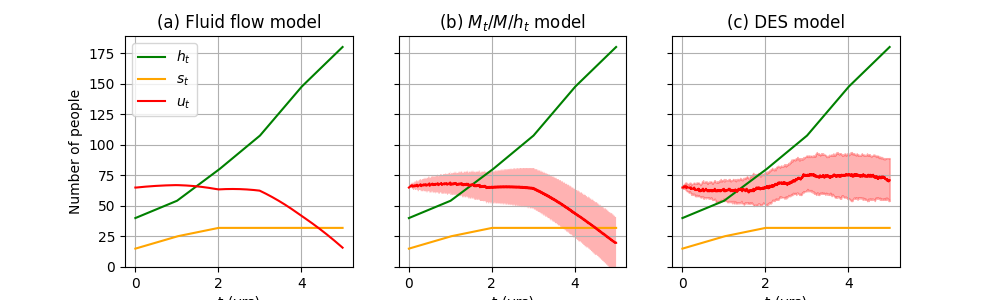
\includegraphics[scale=0.8]{u_t_example.png}
    \caption{Dynamics of $u_d$, $s^D_d$ and $h^D_d$. $n_0 = 12000$, $\mu_0 = 6.106 \times 10^{-4}$, Daily arrival rates $\lambda_d$ in each year: $10.0,11.9,13.1,13.1,11.8$.}
    \label{fig:ut-illustrative}
\end{figure}
%
Figure \ref{fig:ut-illustrative} shows an example of how one might come close to reaching zero unsheltered homelessness in five years.  The level of housing investment steadily increases over time.  There is some initial increase in shelter, though in general there is less investment in shelter over the long term than in housing.  The unsheltered population is stabilized and then eventually decreases approaching zero.  The arrival rates $\lambda_d$ are projected based on a current estimate of 10/day, along with the assumption that arrivals will increase in the coming years due to repercussions of COVID-19.  Eventually, prevention methods will take effect and the arrival rate will hopefully decline \citep{hometogether2022}. The daily service rate $\mu_0$ is equivalent to the mean of a triangular distribution with lower limit $0 \text{ weeks}$, upper limit $400 \text{ weeks}$ and mode $300 \text{ weeks}$.

In Section \ref{do} we will evaluate (\ref{u_t_discrete}) using annual housing and shelter capacity vectors $\boldsymbol{h} = \{h_t \hspace{0.1cm} \forall t \in 0,...,T\}$ and $\boldsymbol{s} = \{s_t \hspace{0.1cm} \forall t \in 0,...,T\}$ where $T$ is a time horizon in years. In this case we assume that any annual increase or decrease in capacity is spread evenly throughout the year, and (\ref{u_t_discrete}) becomes
%
\begin{align} \label{u_t_discrete_h_s_dependent}
u_d(\boldsymbol{h},\boldsymbol{s}) & = n_0 + \sum_{d'=1}^{d} \lambda_{d'} \delta t - \sum_{d'=1}^{d} \mu_0 h^D_{d'}(\boldsymbol{h}) \delta t - h^D_d(\boldsymbol{h}) - s^D_d(\boldsymbol{s}),
\end{align}
%
where 
%
\begin{align} \label{h_d}
h^D_d(\boldsymbol{h}) & = h_{\lfloor{\frac{d}{365}}\rfloor} + \frac{d-\lfloor\frac{d}{365}\rfloor}{365}(h_{\lceil{\frac{d}{365}}\rceil}-h_{\lfloor{\frac{d}{365}}\rfloor})
\end{align}
%
and
%
\begin{align} \label{s_d}
s^D_d(\boldsymbol{s}) & = s_{\lfloor{\frac{d}{365}}\rfloor} + \frac{d-\lfloor\frac{d}{365}\rfloor}{365}(s_{\lceil{\frac{d}{365}}\rceil}-s_{\lfloor{\frac{d}{365}}\rfloor}).
\end{align}
%
This fluid flow model has the advantage of being computationally cheap to run. It is also flexible to incorporate certain real-world system complexities. For example, we could model heterogeneous customer groups in different compartments with different servers, arrival rates and service rates. We could also incorporate re-entries to the system by applying an appropriate discount factor to the third term in Equation \ref{u_t_discrete_h_s_dependent}. 

\subsection{$M(t)/M/h(t)$ queueing model}
%
With an $M(t)/M/h(t)$ queueing model, where $h(t)$ is the time-dependent number of housing servers, we are still modelling the system as illustrated in Figure \ref{fig:simple-q} but we no longer treat arrivals and departures as a fluid, but as individual people. We introduce stochasticity and would like to compute the probability distribution for the number of people housed, sheltered and unsheltered, throughout the time horizon. In doing so we allow a non-zero probability of their being $0$ people in a housing server, thus relaxing the server-always-busy asumption we made with the fluid flow model.

Given the memoryless property of the exponential inter-arrival and service times in an $M(t)/M/h(t)$ queue, we can discretise time and treat this queue as a discrete-time Markov chain where the state space represents the number of people in the system and some large but finite $N$ is the largest possible number in the system. With sufficiently small time intervals of length $\Delta t$, we can assume that within each interval the arrival rate is constant, the number of servers is constant and at most one state change can occur. Therefore, if we know the initial probabilities $p_n(t=0)$ of being in all states $n \in \{0,1,...,N\}$ then for all times $t \in \{0, \Delta t,...,T-\Delta t\}$, we can calculate the probabilities $p_n(t + \Delta t)$ as: 
% 
\begin{align*}
  p_n(t+\Delta t) = & \hspace{0.1cm} p_{n}(t)[1-\lambda(t)\Delta t-\mu_0 m_n(t) \Delta t] \\
                    & + p_{n+1}(t)[\mu_0 m_{n+1}(t) \Delta t] \\
                    & + p_{n-1}(t)[\lambda(t) \Delta t] \\
                    & + \hspace{0.1cm} o(\Delta t) \hspace{1cm} 1 \leq n \leq N-1
\end{align*}
% 
\begin{align*}
  p_0(t+\Delta t) = & \hspace{0.1cm} p_{0}(t)[1-\lambda(t)\Delta t] \\
                    & + p_{1}(t)[\mu_0 m_{1}(t) \Delta t] \\
                    & + \hspace{0.1cm} o(\Delta t)
\end{align*}
% 
\begin{align*}
  p_N(t+\Delta t) = & \hspace{0.1cm} p_{N}(t)[1-\mu_0 m_N(t) \Delta t] \\
                    & + p_{N-1}(t)[\lambda(t) \Delta t] \\
                    & + \hspace{0.1cm} o(\Delta t)
\end{align*}
% 
where $\lambda(t)$ is the arrival rate at time $t$, $\mu_0$ is the service rate of a single housing server and $m_n(t) = \min(n,h(t))$ is the number of busy housing servers when the system is in state $n$ at time $t$. The bias in the results introduced by using constant values in each time interval for $\lambda(t)$ and $h(t)$ vanishes as $\Delta t \to 0$. The probabilities $p_n(t)$ can then be analysed to estimate the expected number of people housed, sheltered and unsheltered, throughout the time horizon. For example, the expected number unsheltered at time $t$ is given by:
%
\begin{align} \label{u_t_mmt}
\mathbb{E}[u(t)] & = \sum_{n=0}^{N} p_n(t) \max(0,n-h(t)-s(t)), 
\end{align}
%
where $s(t)$ is the time-dependent number of shelters. This model is more computationally costly than the fluid flow model, but still cheap compared to a discrete-event simulation model. We have introduced stochasticity and allowed housing servers to be empty with some positive probability, but we are still limited in what real-world complexity we can model. Our choice of distribution for inter-arrival times and service times is also limited to the exponential distribution. 
%
\subsection{Discrete-event simulation model} \label{DES}
%
Discrete-event simulation (DES) is a form of stochastic simulation which models the evolution of a complex system according to a chronological event list which is updated throughout the simulation. DES is a powerful modeling tool given its ability to incorporate bespoke system complexities. It also naturally accomodates stochasticity by using a stream of $\text{Uniform}(\text{min} = 0, \text{max} = 1)$ pseudo-random numbers to drive the generation of random variates for model variables such as inter-arrival and service times. The drawback of DES is its computational cost which arises from the need to step through each event which occurs within the modelled system over the time horizon.

We have developed a DES model of our homelessness care system, which is a Python version of the DES model of \cite{singham2023discrete}, built in Simio. In this model, shelter acts as a server, giving rise to a tandem queueing system, as illustrated in Figure \ref{fig:des-q}. A proportion of those leaving housing re-enter the system, as illustrated, and the exponential and triangle distributions are used for inter-arrival and housing service times, respectively. 
%
\tikzstyle{server_s} = [rectangle, rounded corners, minimum width=0.5cm, minimum height=1cm,text centered, draw=black, fill=gray!30]
\tikzstyle{server_h} = [rectangle, rounded corners, minimum width=0.5cm, minimum height=1cm,text centered, draw=black, fill=teal!30]
\tikzstyle{arrow} = [thick,->,>=stealth]
%
\begin{figure}
  \begin{center}
    \begin{tikzpicture}
      \node (start) [empty, align=center] {};
      \node (shelter) [server_s, right of=start, xshift=3cm] {Shelter};
      \node (housing) [server_h, right of=shelter, xshift=3cm] {Housing};
      \node (end) [empty, right of=housing, xshift=1.4cm, align=center] {};
      \draw [arrow] (start) -- node [above] {Unsheltered} (shelter);
      \draw [arrow] (shelter) -- node [above] {Zero buffer}(housing);
      \draw [arrow] (housing) -- node [above] {}(end);
      \draw [arrow] (housing) to [out=210,in=330] node [below] {Partial re-entry}(shelter);
    \end{tikzpicture}
    \caption{Tandem queueing system with re-entries} \label{fig:des-q}
  \end{center}
\end{figure}

While this is still a relatively simple DES model, it provides the framework for us to add many more system complexities should we so desire. For example, we could model the non-zero time needed to occupy a house with a new resident following the departure of its previous resident. We could also model the process of conversion of shelter to housing, which is a strategy proposed by Alameda County to improve services in the long term. We thus treat our DES model as a high-fidelity model, capable of the highest level of modelling accuracy, in comparison to our low- and medium-fidelity models, albeit at a computational cost.

\newpage

\section{Deterministic optimisation with low-fidelity model} \label{do}
%
In this section, we will present an optimisation formulation applied to our deterministic fluid flow model. This formulation will optimise the levels of housing and shelter to be built over time, and the objective function wilfl attempt to minimise the unsheltered and sheltered population over the modelling horizon. Aside from the obvious need for cost constraints, we improve the real-world feasibility of our solutions by incorporating policy-based shape constraints on the housing and shelter capacities, which are functions of time. For example, though it would be better from a queueing standpoint to spend all financial resources upfront, the reality is that investment from the taxpayer will likely ramp up over a period of years. Furthermore, though their is political appetite for the use of emergency shelter in the short term, this is not seen as a sustainable long-term solution, so we introduce a unimodal shape constraint on the shelter capacity function. To the best of our knowledge, this is the first time long-term capacity planning is addressed by constructing and optimisng a tractable fluid flow model. 
%
\subsection{Optimisation formulation} \label{opt}
%
First, we present the basic notation associated with the terms in our formulation. The associated numerical results will be presented in Section \ref{results}. We define the following terms:

\begin{itemize}
\item Let subscript $d$ denote time in days and subscript $t$ denote time in years.
\item Let $T_a$ be the horizon (in years) over which we model the dynamics of the system while altering housing and shelter capacities, where $T_a \in \mathbb{N}$. %\LRL{Could use $\mathbb{N}$ instead of $Z^+$.} \GB{Done}
\item Let $T_b$ be the additional horizon (in years) over which we continue to model the dynamics of the system without altering housing or shelter capacities, where $T_b \in \mathbb{N}$. We do this in order to allow increased housing capacity to have a meaningful effect on the system over a long period of time beyond a finite investment period. %\LRL{Should we have an explicit statement about why we continue to study the system on a time horizon beyond our decision making horizon? Otherwise it might seem like a slightly odd thing to do.} \GB{Done}
\item Let $D=(T_a+T_b)\times365$ be the total modeling horizon in days.
\item The vectors $\boldsymbol{h} = \{h_t \hspace{0.1cm} \forall t \in 0,...,T_a+T_b\}$ and $\boldsymbol{s} = \{s_t \hspace{0.1cm} \forall t \in 0,...,T_a+T_b\}$ are the model decision variables which contain continuous-valued annual housing and shelter capacities, respectively. The fluid flow model spreads annual changes in capacity equally over each day in the year, as detailed in equations (\ref{h_d}) and (\ref{s_d}).
\item $C$ is the total budget for building housing and shelter. \par
\item Let $c_h$ and $c_s$ be the costs of increasing $h_t$ and $s_t$, respectively, by 1, at any time.
\item Let $H_0$ and $S_0$ be the initial housing and shelter capacities, respectively.
\item Define $w \in (0,1)$ as a weight between two objective terms which ensures that a sheltered queue is not penalized more than an unsheltered queue of the same size.
\end{itemize}

Recall that $u_d$ and $s_d$ are the output of the fluid flow model reporting the unsheltered and sheltered populations each day, respectively.  Let $y(\boldsymbol{h},\boldsymbol{s})$ be a deterministic quadratic objective function, evaluated using the fluid flow model equations (\ref{u_t_discrete_h_s_dependent}), (\ref{h_d}) and (\ref{s_d}). We use a quadratic objective function to reflect the fact that neither the unsheltered nor the sheltered queue should become excessively long. Finding this balance involves a careful trade-off between building shelter (which quickly reduces the unsheltered queue) and building housing (which gives long term relief to the system, at the expense of initially large unsheltered queues). Furthermore, as seen in Alameda County, long waiting times can increase subsequent service times as people's situations may deteriorate. This further motivates the quadratic penalty on both parts of the queue.
%
\begin{align} \label{y}
  y(\boldsymbol{h},\boldsymbol{s}) = \frac{1}{D} \sum_{d=1}^{D} u_d(\boldsymbol{h},\boldsymbol{s})^2 + \frac{w}{D} \sum_{d=1}^{D} s^D_d(\boldsymbol{s})^2.  
\end{align}
%
We now introduce policy-based shape constraints. First, we ensure that the rate of housing capacity increase must stay the same or increase over $T_a$ to reflect the fact that budget available for housing capacity expansion may typically grow over time and not all be available immediately. This not only requires housing to increase over time, but the rate of change must increase as well, which amounts to an increasing derivative shape constraint.

We can also require shelter investment to follow a unimodal function, whereby it increases for a given time period, and then decreases.  This shape constraint has been suggested by Alameda County as a way of encouraging an initial ramp-up of shelter, but eventually excess shelter could be converted to housing to avoid permanent large shelters once the queue has been reduced.  To implement this unimodality constraint on $s_t$, we introduce a mode $T_c$ for the shelter capacity function over time, where $T_c \leq T_a$ and $T_c \in \mathbb{N}$. We ensure that the shelter capacity monotonically increases before $T_c$ and monotonically decreases subsequently. Decreases in the shelter capacity correspond to shelter being decomissioned - in this case the money saved may be spent on housing. The non-linear formulation including this unimodal shape constraint and rate of change constraint is:
%
\begin{eqnarray}
        \Phi = & \min_{\boldsymbol{h},\boldsymbol{s}} y(\boldsymbol{h},\boldsymbol{s})\label{p2c0} & \\
        \text{ s.t. } & \sum_{t=1}^{t'} c_{h}[h_{t}-h_{t-1}] + c_{s}[s_t-s_{t-1}] \leq C & \forall t' \in \{1, ..., T_a\}\,\quad \quad\label{p2c1}\\
        & h_0 = H_0 & \label{p2c2} \\
        & h_{t} \geq h_{t-1} & \forall t \in \{1,...,T_a\}\, \quad \quad\label{p2c3}\\   
        & h_t = h_{T_a} & \forall t \in \{T_a+1,...,T_a+T_b\}\, \quad \quad \label{p2c4} \\
        & h_{t+1} - h_{t} \geq h_{t} - h_{t-1} & \forall t \in \{1,...,T_a-1\}\, \quad \quad\label{p2c5} \\    
        & s_0 = S_0 & \label{p2c6} \\
        & s_{t} \geq s_{t-1} & \forall t \in \{1,...,T_c\}\, \quad \quad\label{p2c7} \\
        & s_{t} \leq s_{t-1} & \forall t \in \{T_c+1,...,T_a\}\, \quad \quad\label{p2c8} \\ 
        & s_t \geq s_0 & \forall t \in \{T_c+1, ..., T_a\}\, \quad \quad \label{p2c9} \\
        & s_t = s_{T_a} & \forall t \in \{T_a+1,...,T_a+T_b\}. \quad \quad \label{p2c10}
\end{eqnarray}
%
Constraints (\ref{p2c1}) ensure the total budget is never exceeded. A single budget constraint is not enough, since then the total budget could be exceeded in one year as long as a saving was subsequently made from decommissioning shelter. With this set of constraints we ensure that at no point can the total expenditure to that point exceed the total budget, so any savings from decommissioning shelter cannot be spent before they are made. Constraints (\ref{p2c2}) and (\ref{p2c6}) enforce the initial housing and shelter capacities. Constraints (\ref{p2c3}) ensure the housing capacity monotonically increases, while constraints (\ref{p2c5}) ensure the rate of change of housing capacity also monotonically increases from year to year. Constraints (\ref{p2c7}) ensure the shelter capacity monotonically increases up to the mode $T_c$ and constraints (\ref{p2c8}) ensure it subsequently decreases monotonically. Constraints (\ref{p2c9}) ensure the shelter capacity never drops below its initial capacity. Finally, constraints (\ref{p2c4}) and (\ref{p2c10}) fix $h_t$ and $s_t$ during the horizon $T_b$ after the building horizon has occurred.
%
\subsection{Numerical results} \label{results}

In Table \ref{tab:model_params} we list the model parameters we used when optimising formulations $\Phi$. These approximate values are taken from \cite{hometogether2022} and \cite{singham2023discrete}. We choose $w$ to be sufficiently high to give a meaningful penalty to shelter but without undermining its advantage over an unsheltered queue. Additionally, while we use a current estimate of the arrival rate of 10/day for the first $T_a$ years of the modeling horizon, we anticipate with major local prevention efforts \citep{RICActionPlan}, the arrival rate could potentially drop significantly to an estimate of 6/day.

\begin{table}
        \begin{center}
        \caption{Model parameters}
        \begin{tabular}{ |c|c| } 
         \hline
         \textbf{Parameter} & \textbf{Value ($\Phi$)}\\ 
         \hline
         $T_a$ & $5 \text{ years}$\\ 
         \hline
         $T_b$ & $5 \text{ years}$\\
         \hline
         $T_c$ & $3 \text{ years}$\\          
         \hline
         $\lambda_d$ & $\frac{10}{day} \hspace{0.1cm} \forall d \in \{1,...,T_a\times365\}$\\ 
          & $\frac{6}{day} \hspace{0.1cm} \forall d \in \{T_a\times365+1,...,D\}$\\          
         \hline           
         $X_0$ & 12,000 people\\         
         \hline
         $h_0$ & 4,000 units\\ 
         \hline
         $s_0$ & 1,500 units\\ 
         \hline      
         $c_h$ & 30,000 USD/unit\\ 
         \hline
         $c_s$ & 10,000 USD/unit\\ 
         \hline         
         $C$ & 200,000,000 USD\\ 
         \hline  
         $\mu_0$ & $6.106 \times 10^{-4}$/day \\ 
         \hline
         $w$ & $0.3$\\ 
         \hline
        \end{tabular}
        \label{tab:model_params}
        \end{center}
        \end{table}

In Figure \ref{fig:phi2opt} we illustrate the model dynamics for the optimal solution to $\Phi$, which involves the building of a mixture of extra housing and extra shelter. The quadratic penalty associated with a high unsheltered population encourages shelter which quickly reduces the size of the unsheltered queue. However, the quadratic penalty of having a large sheltered population encourages investment in housing. This housing investment in time also has a meaningful effect on reducing the unsheltered queue, since sufficient houses may be built to have a total service rate higher than the arrival rate, thus bringing stability to the system. 
%
\begin{figure}[h!]
    \centering
    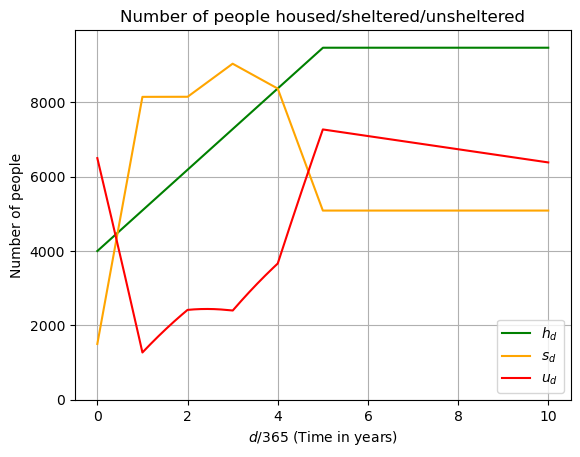
\includegraphics[scale=0.8]{phi2-opt.png}
    \caption{Optimal solution for $\Phi$.}
    \label{fig:phi2opt}
\end{figure}

We can see the effect of shape constraints. We note that the initial ramp up of shelter is able to bring the unsheltered queue down in the short term. The rate of increase in the housing capacity must not decrease over time so we see a more steady increase in housing compared to previous solutions. The total amount of housing we can build is affected by the fact that after the shelter mode at $t=3$ years, decommissioning shelter makes more budget available for housing. Thus we are able to achieve sufficient housing for a stable system in the long-term, while affording immediate relief to the system via shelter. We note that with this formulation, for every $3$ shelters decommissioned, $1$ house may be acquired, resulting in $2$ people immediately rejoining the unsheltered part of the queue. Although this enables the housing capacity to increase which is good for long-term relief to the system, the immediate effect is undesirable in practice and we see that after $5$ years the unsheltered queue is again very large. An alternative formulation may enforce a more controlled decommissioning process by, for example, including a shape constraint on the total number of housing and shelter units.      
\begin{figure}[h!]
    \centering
    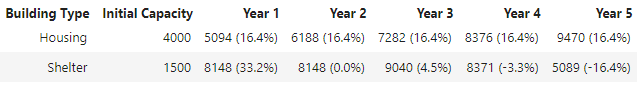
\includegraphics[scale=0.8]{results_comparison.png}
    \caption{Optimal capacity per year (Proportion of total budget spent per year)}
    \label{tab:phi1phi2results}
\end{figure}

In Figure \ref{tab:phi1phi2results} we detail the optimal solution to $\Phi$ in terms of the capacity at the end of each year and the proportion of the total budget spent on building in that year. Negative budget spent corresponds to a saving made by decommissioning shelter. The optimal solution spends the maximum possible budget of 200,000,000 USD. The solution sees a large early ramp up of shelter and a steady investment in housing over time. In years $4$ and $5$ we see decommissioning of shelter to enable the continued investment in housing. 

We solved this problem in $0.759$ seconds using the IPOPT solver in Pyomo. All code used for this analysis is publicly available \href{https://github.com/grahamburgess3/psor-paper-housing}{on GitHub}.

\subsection{Determinsitic optimisation: discussion} \label{do-discuss}

Most capacity planning optimisation formulations we have reviewed in the literature (e.g. in runaway homeless youth systems) consider capacity expansion from a single-stage perspective, in that the decision maker has one shot to choose and optimize a fixed capacity to accommodate the queueing system.   In reality, most public sector services do not have the resources to instantaneously ramp up to the ideal capacity, as there may be budgetary or time constraints that control this rate.  A model that accounts for these limits in capacity expansion over time will provide a more realistic and executable plan, hence we attempt to provide a method for determining how to allocate resources over time.

While housing is the primary resource and is modeled as the main server system, we also model investment into shelter, which supports some of the people in the queue, while not modeled as a server. Our quadratic objective function is able to balance the desire for high levels of housing at high cost against cheaper shelter options. In addition to budgetary constraints, we employ shape constraints as a means of ensuring our investment function output is feasible from a policy-making and implementation standpoint.  The idea of a unimodal function for shelter investment has been suggested by Alameda County, and such shape constraints can easily be implemented in our framework.

There are many opportunities for alternative formulations.  Smoothness constraints on the unimodal shelter capacity function may give more practical solutions that appear reasonable to constituents. Further constraints to control the decommissioning of shelter may also be appropriate. A bi-objective formulation would likely give further insight into the trade-off between short-term relief to the system via shelter and long-term relief via housing. Alternatively, a goal programming formulation which penalised deviations from a time-dependent goal on the unsheltered population would be interesting to explore.

We have here performed deterministic optimisation using a low-fidelity fluid flow model. This has enabled us to develop and explore an optimisation formulation which captures the key objectives, trade-offs and constraints. It has also enabled us to quickly get a feel for the nature of good solutions to the time-dependent capacity planning problem using a simple model. The natural next step is to develop a simulation optimisation model which accounts for stochastic uncertainty.

\newpage

\section{Discussion of uncertainty} \label{uncert}

Our optimisation in Section \ref{do} assumes that we know the future arrival rates of homeless people into the homeless care system, and that we know their service times in housing. The fluid flow model projects forward the resulting unsheltered queue based on these exact quantities. In reality, actual inter-arrival times (or service times) are realisations of some unknown true distribution which we can only estimate using information available to us. Even if we knew the true distributions, we would not know what the next inter-arrival time (or service time) would be, due to the random nature of these processes. These aspects of uncertainty pervade all long-term capacity planning problems and it is therefore important that we consider them as we move forward to consider simulation optimisation.

As discussed in Section \ref{models}, a stochastic simulation can offer a high-fidelity model of a queueing system. It incorporates the stochasticity in inter-arrival and service times, and it allows us to capture certain important real-world complexities. There are two types of uncertainty in stochastic simulation: input uncertainty and stochastic uncertainty. Input uncertainty arises from not knowing the true input models for, say, inter-arrival and service times. Stochastic uncertainty arises from only simulating a finite amount of random variates from the input models. The latter can be mitigated by performing many simulation replications. The former is typically mitigated by bootstrapping from the data used to fit the input models, to fit new input models which can be used to generate new random variates in new simulation replications.

The relative importance of input and stochastic uncertainty varies when modelling different systems. If service times are long, such as in housing or prison models, then the stochastic uncertainty may be less important; one is more interested in high input uncertainty stemming from knowing neither future population demands nor service rates even for today's customers. If service times are short, such as in many healthcare applications, service time input models are typically more accurate and the stochastic uncertainty becomes more important. 

Simulation optimisation suffers from both input uncertainty and stochastic uncertainty as a direct result of using stochastic simulation to model system performance. The main focus of this PhD research, at least initially, will be multi-fidelity simulation optimisation (MFSO) where we do not consider input uncertainty. We do, of course, consider stochastic uncertainty, which is a defining feature of stochastic simulation and simulation optimisation. This is an appropriate first step for a couple of reasons. Firstly, the initial research challenges (discussed in Section \ref{mfso}) are challenging enough without input uncertainty. Secondly, stochastic uncertainty is relatively important in many long-term capacity planning problems, especially when service times are short, such as in many healthcare problems. 

We do here acknowledge that for the homeless care system, there are extremely high levels of input uncertainty. Even if we fitted input models for inter-arrival and service times using extensive historic data, we would still be highly uncertain of whether these models would accurately predict future inter-arrival and service times. This is because they are connected with other events which are highly unpredictable such as house prices, political decisions and global health and climate emergencies. It may be that input uncertainty is more important than stochastic uncertainty in this particular setting which motivates further research of input uncertainty in MFSO methods. 

\newpage

\section{Potential research contributions} \label{mfso}

The next steps of this PhD research will address current challenges at the intersection of integer-ordered and multi-fidelity SO. An integer-ordered SO approach is naturally applicable to long-term public sector capacity planning problems since decision variables are often the number of units of resource to make available. Multi-fidelity methods are also attractive in this area given the availability of suitable multi-fidelity queueing models. We discuss below some initial ideas for contributing to the literature at the intersection of these active fields of research. We conduct this reseach in the spirit of exploring to what extent these methods can give meaningful analytical support to decision makers in the public sector.

Gradient-based integer-ordered SO methods such as DSA and R-SPLINE expend substantial simulation effort in estimating gradients on the continuous domain. For a given point on the $d$-dimensional continuous domain, to estimate the gradient, all $(d+1)$ integer points on the surrounding simplex must be simulated multiple times. This could be more efficient by using information from low-fidelity models. One could, for example, use solely a low-fidelity model for objective function estimation at points on the simplex. Alternatively one could use a meta-model defined as a combination of a low-fidelity model and an error term, using some simulation effort to fit this meta-model.

GMRF-based integer-ordered SO methods are popular in the literature but are hampered by the computational expense of inverting the conditional precision matrix which is needed to update the conditional distribution. Some efforts to address this problem aim to reduce the number of times a full inversion is required. For example, the `rapid' GMIA algorithm (rGMIA) of \citep{semelhago2021rapid} constructs a `promising set' of solutions and efficiently searches in this set for some time by updating only the relevant parts of the conditional distribution. This leads to considerable efficiencies, but it does not involve the use of multi-fidelity model information.

The multi-fidelity GMIA algorithm (MFGMIA) of \citep{li2022multi} adds a new `layer' of nodes to the GMRF graph for each low-fidelity model available. Each high-fidelity solution is connected to all of its low-fidelity counterpart nodes with an edge. The precision matrix and the resulting conditional distribution are designed to control the influence given to each low-fidelity model for each solution, based on the quality of each low-fidelity model and on the amount of high-fidelity simulation effort expended for each solution. These are good ideas, however there are still problems and room for improvement. Firstly, it is assumed that low-fidelity information for all feasible solutions is available from the start without cost, which is problematic if low-fidelity models do incur cost and/or if the solution space is very large. Secondly, the prior distribution for the GMRF is still a constant across the entire solution space for each model which does not use multi-fidelity information to its full potential.

Our research may build upon the ideas of MFGMIA by transferring concepts from multi-fidelity sequential kriging optimisation (MFSKO) \citep{huang2006sequential} where the cost of low-fidelity information is accounted for and their is heirarchy amongst the low-fidelity models. A key idea is to explore the possibility of using low-fidelity information to bring structure to the prior distribution, without requiring low-fidelity evaluation of the entire solution space. We may also merge ideas from rGMIA and MFGMIA to use low-fidelity information to help identify promising sets. We may also draw on information-theoretic concepts from multi-fidelity batch BO such as the use of entropy-based acquisition functions. Finally, we may expand the application of GMRFs to include modelling the error of low-fidelity models, again using concepts from MFSKO but on a discrete solution space.

We plan to extend our MFSO research by considering one or both of the following research challenges which arise when applying MFSO methods to long-term public sector capacity planning problems. First is the question of input uncertainty which can overshadow stochastic uncertainty as discussed in Section \ref{uncert}. Standard methods of bootstrapping from input data are not suitable since this uncertainty does not arise due to a lack of data but due to genuine uncertainty regarding the complex factors which could affect future arrival or service rates. An optimisation approach which considers a range of possible input models may prove appropriate. We might consider a range of input distribution classes as well as a range of input model parameters.

Secondly, with long planning horizons, decision makers typically revisit and adjust their plans on a regular basis, in light of new information. A dynamic optimisation approach may therefore be appropriate to consider. For example, suppose we require a $T$-year plan where $T>1$. We might first use MFSO with the known current system state to propose a plan for the next $L$ years where $1<L<T$. We might then simulate the system for a year assuming we follow the proposed plan for the first year, and observe the resulting simulated system state. We could then optimise again with MFSO for the next $L$ years based on the simulated system state after one year. By repeatedly simulating for a year and re-optimising we could obtain a $T$-year plan which incorporated the dynamic element of the decision-making process. Of course many replications would be needed to establish a good plan with a method like this, given the randomness associated with simulating the system with the first year of a proposed plan.

\newpage

\bibliographystyle{apalike}
\bibliography{bibliography.bib}

\end{document}